\documentclass[a4paper]{report}
\usepackage{ngerman}
\usepackage{graphicx}
\usepackage{subfig}
\usepackage[svgnames]{xcolor} % Required for colour specification
\newcommand*{\plogo}{\fbox{$\mathcal{PL}$}} % Generic dummy publisher logo
\renewcommand{\baselinestretch}{1.25}
\usepackage[T1]{fontenc} % Output font encoding for international characters
\usepackage[utf8]{inputenc} % Required for inputting international characters
\usepackage{tgadventor} % Use the Paratype Serif font
\renewcommand{\familydefault}{\sfdefault}
\usepackage{float}
\usepackage[hidelinks]{hyperref}
\usepackage{refstyle}
\usepackage{caption}
\usepackage{pdfpages}%
\usepackage{geometry}
 \geometry{
 left=30mm,
 top=30mm,
 bottom=20mm,
 }

\usepackage{fancyhdr}
\pagestyle{fancy}
\fancyhf{}
\rhead{Overleaf}
%\lhead{\LaTeX{} tutorials}
\lhead{\nouppercase{\rightmark} (\nouppercase{\leftmark})}
\rfoot{Page \thepage}
\renewcommand{\headrulewidth}{2pt}

	%------------------------------------------------
	%	Start der Beschreibung
	%------------------------------------------------
\begin{document}


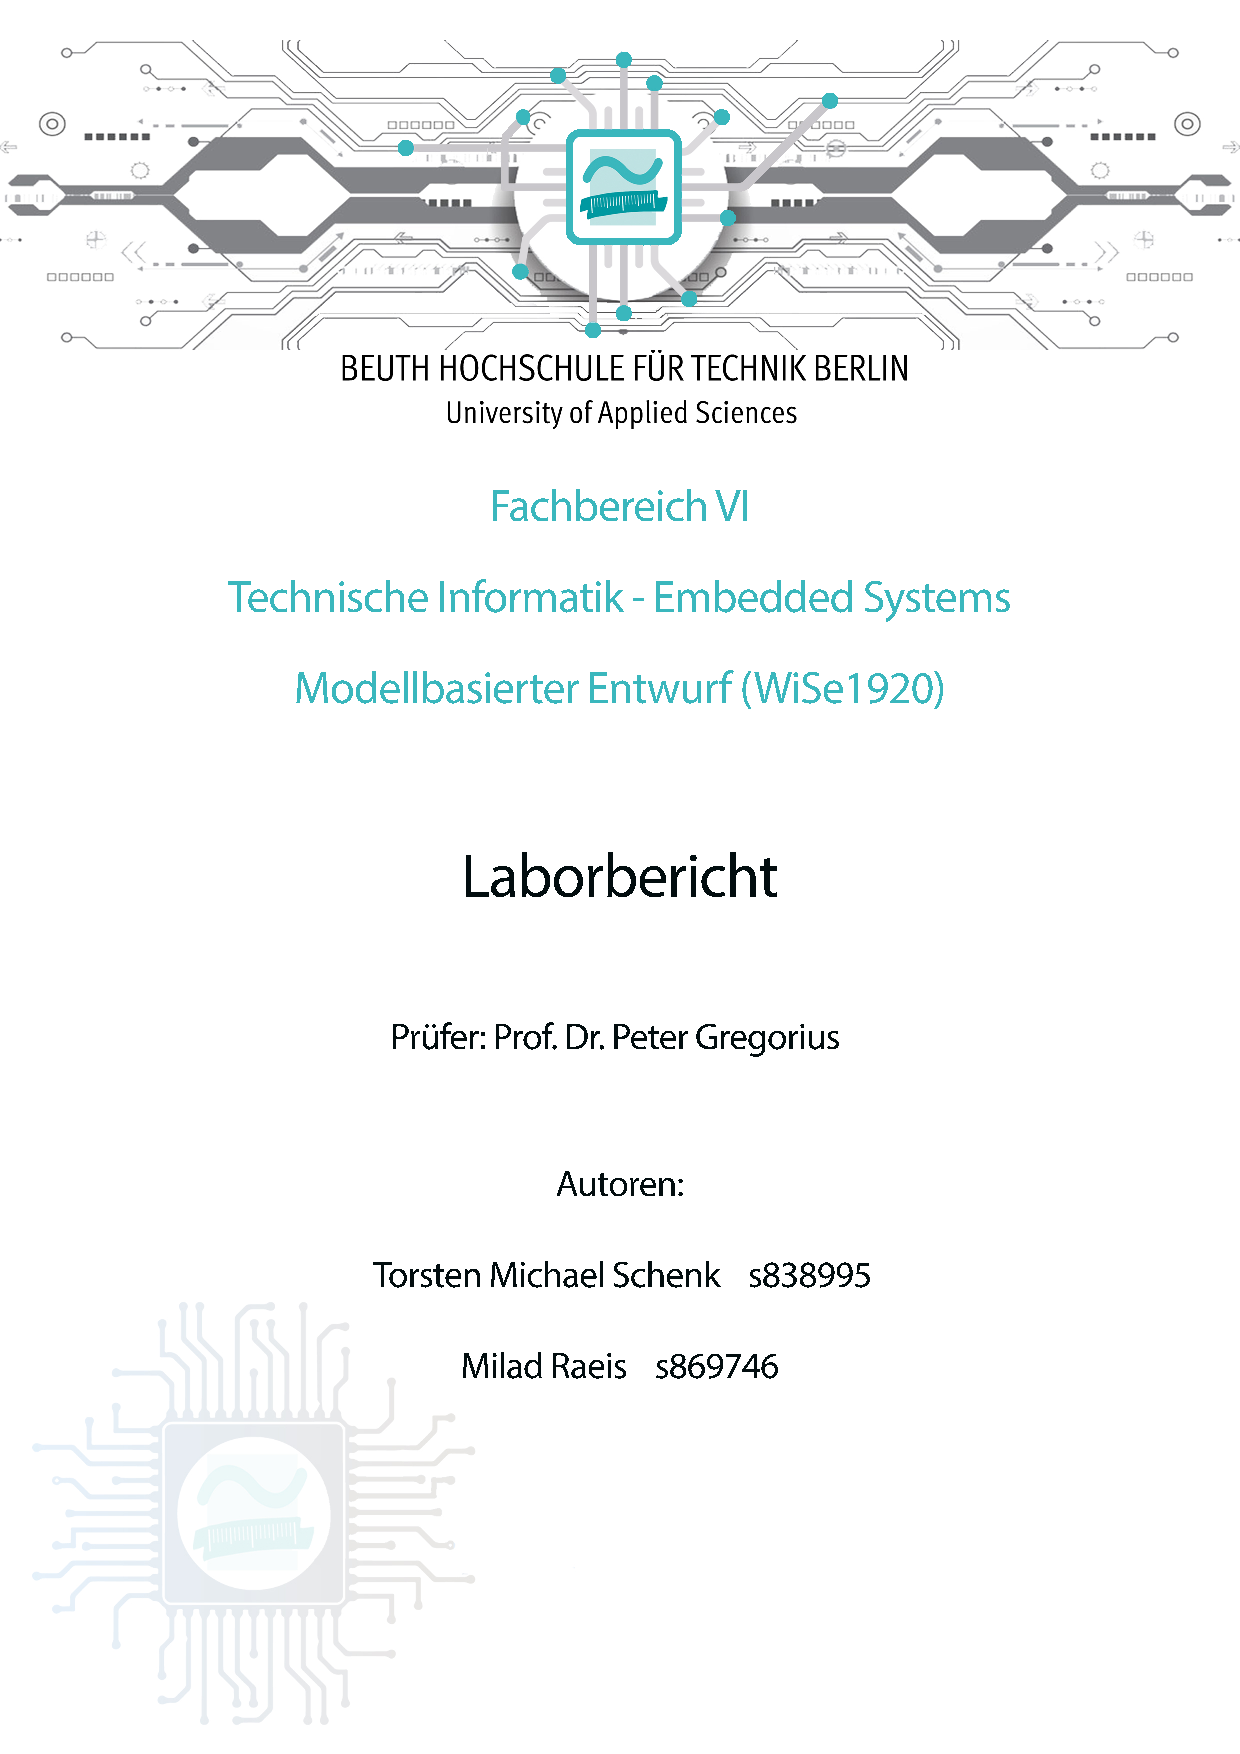
\includepdf{Coverpage.pdf}
\tableofcontents
\listoffigures



	%------------------------------------------------
	%	1. Chapter
	%------------------------------------------------


\chapter{Einleitung}
*********************************************************************************************
*************************
***************************************************
********************************************
************************************************************
******************************************************
************************************************



	%------------------------------------------------
	%	2. Chapter
	%------------------------------------------------

\chapter{Hardware}

In diesem Kapitel werden die für das Projekt erforderliche Hardware ermittelt und erläutert.\\

Nachfolgend zeigen wir den Überblick über unser Projekt: 

	\begin{figure}[H]
	\centering
	\subfloat{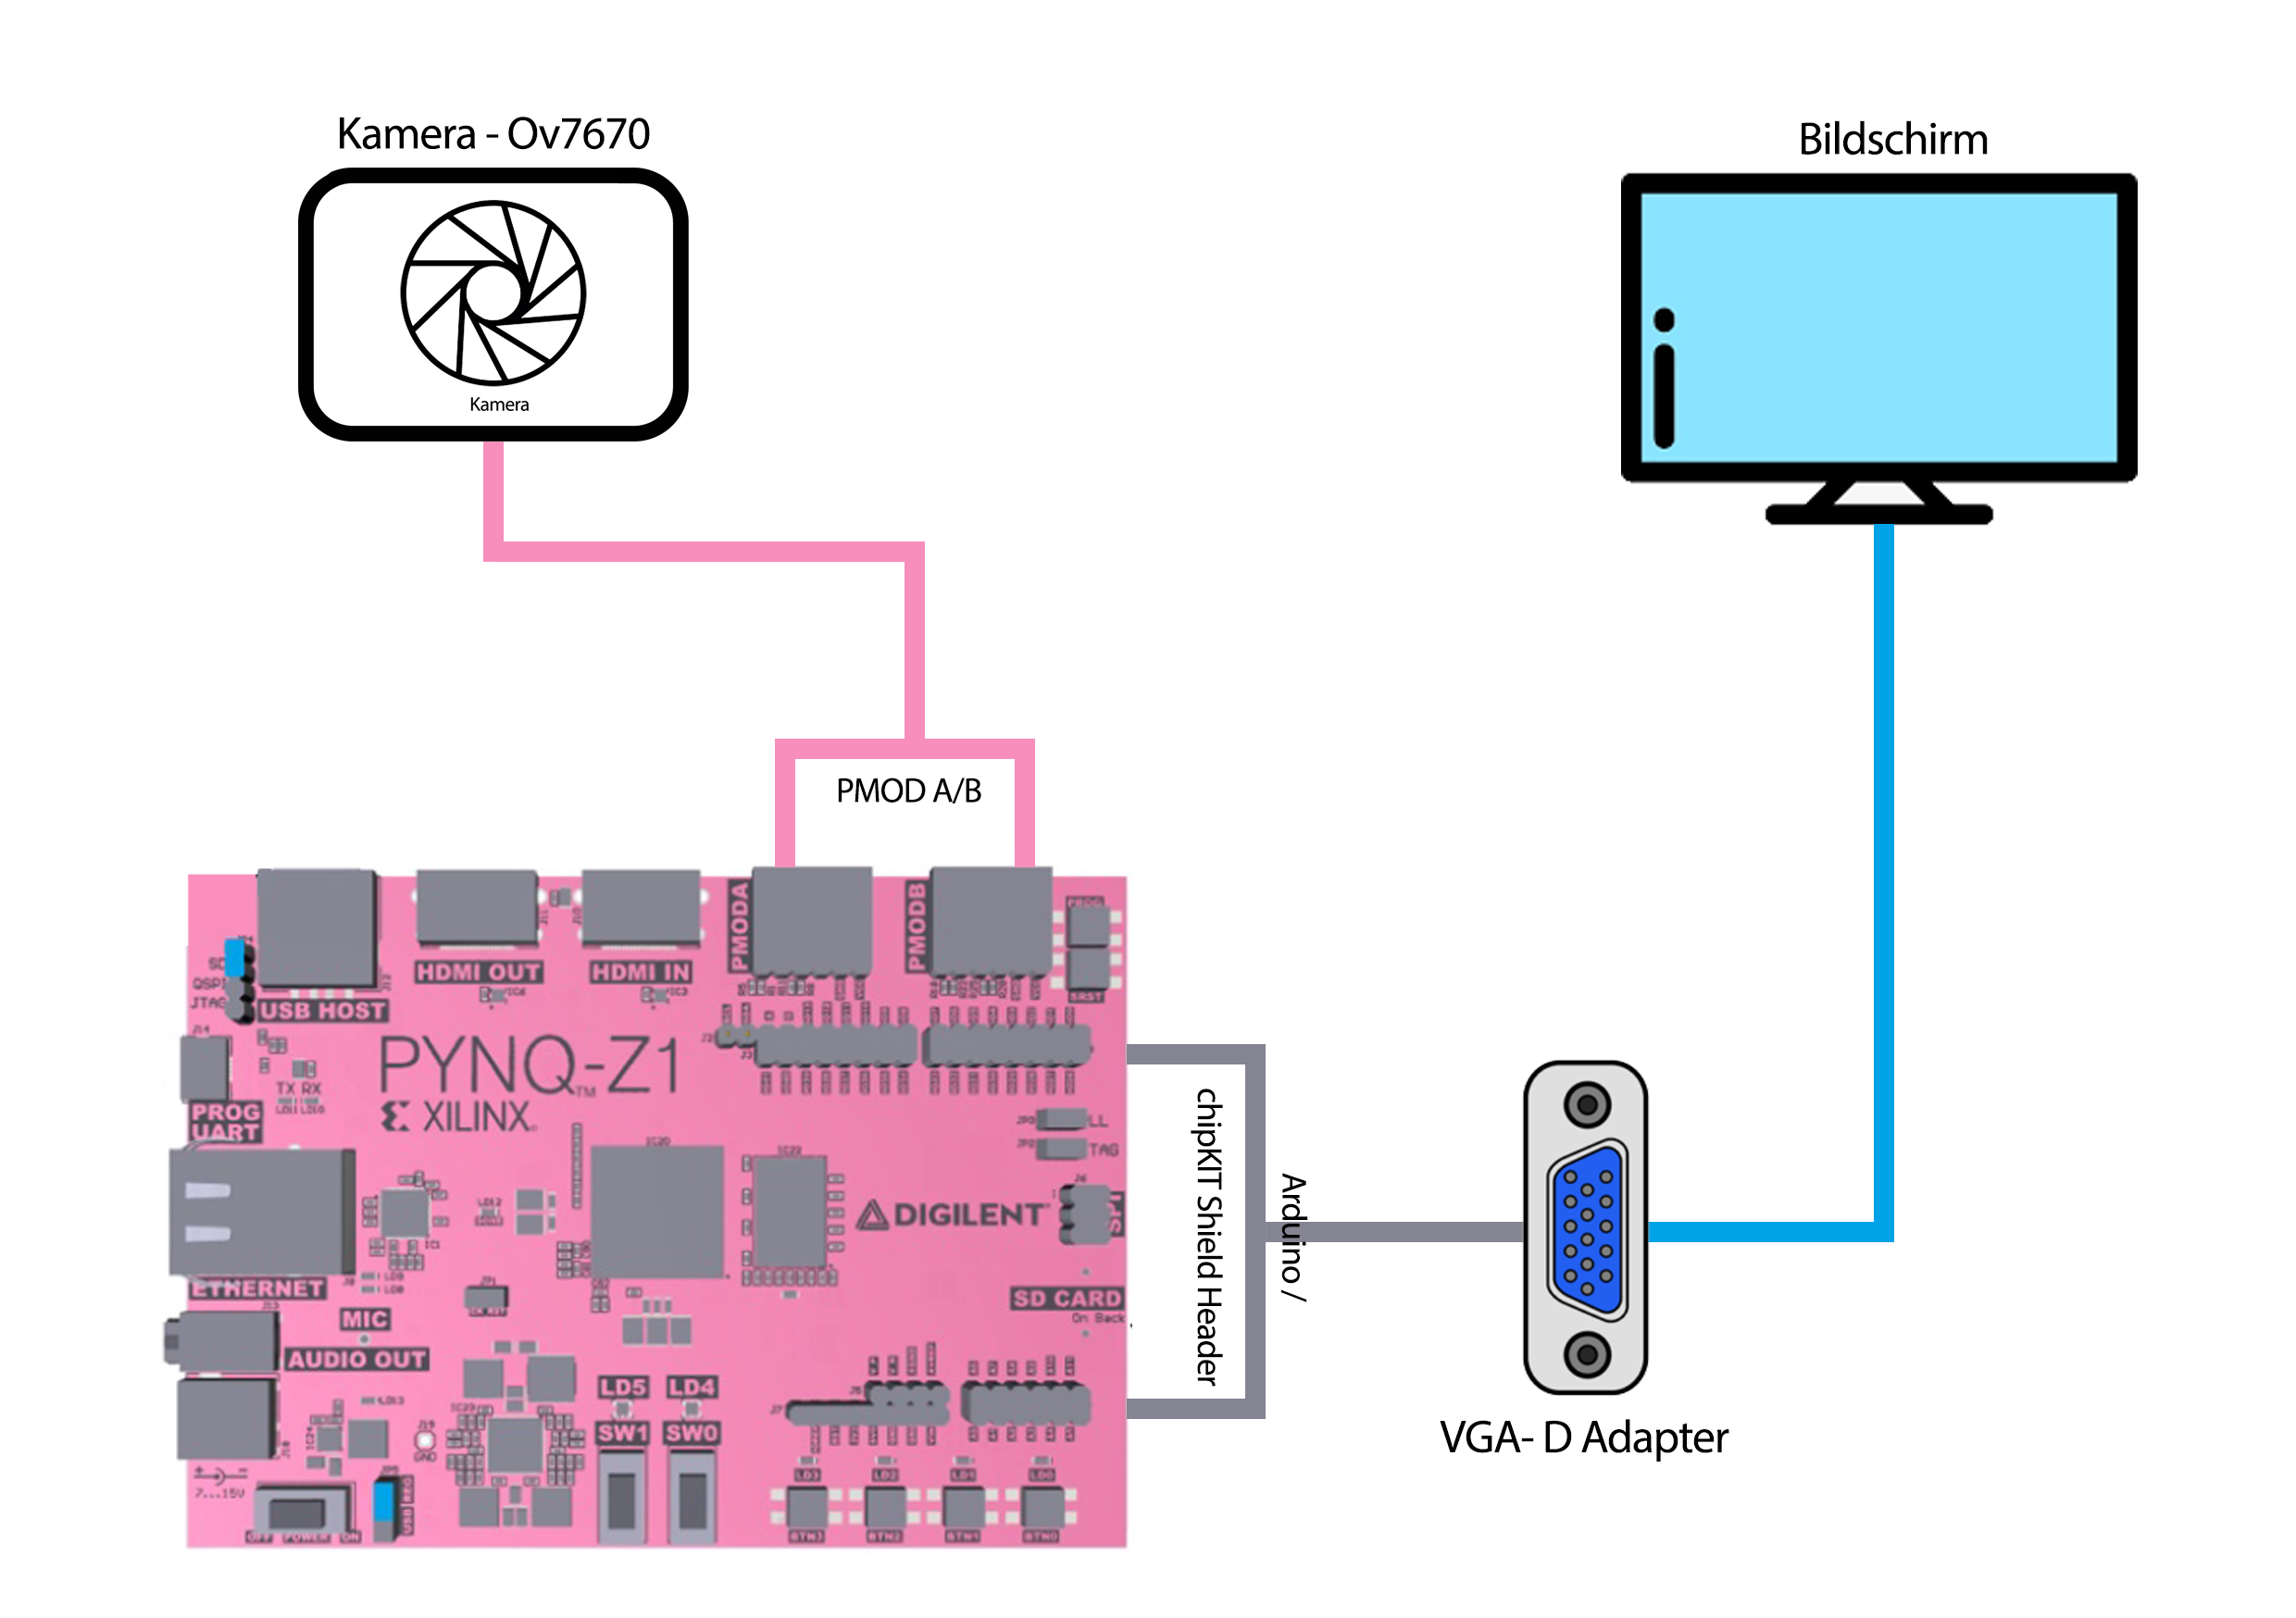
\includegraphics[width=13cm,height=8cm]{PIC/schematik}}
	\caption{Entwurf des Projects}
	\label{Entwurf des Projects}
	\end{figure}



\section{Xilinx Pynq-Z1 board}
Das PYNQ-Z1 Board wurde für die Verwendung mit PYNQ entwickelt, einem neuen Open-Source-Framework, das es Embedded-Programmierern ermöglicht, die Fähigkeiten von Xilinx Zynq All Programmable SoCs\footnote{System On Chip} (APSoCs) zu nutzen, ohne programmierbare Logikschaltungen entwickeln zu müssen. Die programmierbaren Logikschaltungen werden als Hardwarebibliotheken importiert und  ihre APIs\footnote{Application Programming Interface} sind im Wesentlichen so programmiert, dass sie  wie die Softwarebibliotheken importiert und programmiert werden. Für Designer, die das Basissystem mit neuen Hardware-Bibliotheken erweitern wollen, stehen die Xilinx Vivado WebPACK-Tools kostenlos zur Verfügung.

Das PYNQ-Z1 unterstützt Multimedia-Anwendungen mit integrierten Audio- und Videoschnittstellen und ist so konzipiert, dass es unkompliziert mit Pmod-, Arduino- und Grove-Peripheriegeräten sowie universellen IO-Pins erweiterbar ist.
Ebenso kann das PYNQ-Z1 Board auch mit USB-Peripheriegeräten wie WiFi, Bluetooth und Webcams erweitert werden und ist die Hardware-Plattform für das PYNQ Open-Source-Framework.


	\begin{figure}[H]
	\centering
	\subfloat{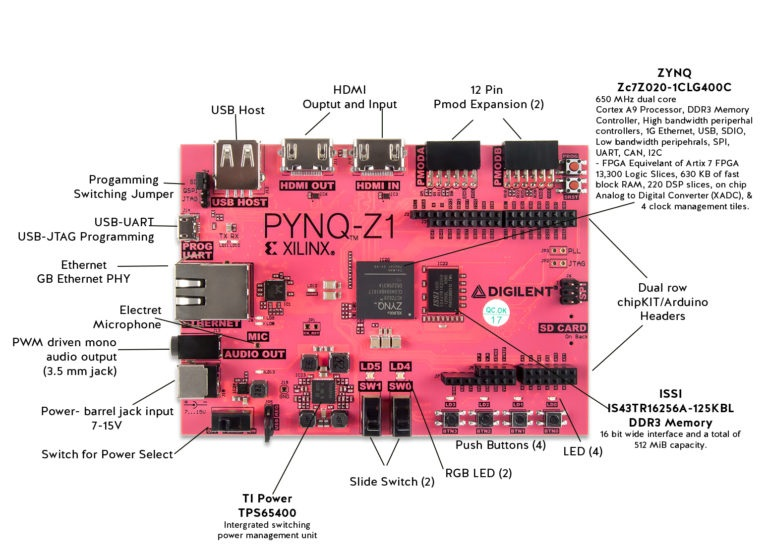
\includegraphics[width=14cm,height=9cm]{PIC/PYNQZ1}}
	\caption{Übersicht PYNQ-Z1}
	\label{Übersicht PYNQ-Z1}
	\end{figure}

Hier beschreiben wir mensche die Eigenschaften des Boards:

	\begin{enumerate} 
	\item 512 MB DDR3 mit 16-bit Bus bei 1050Mbps.
	\item 650 MHz Dual-Core Cortex-A9 Prozessor.
	\item 16 MB Quad-SPI\footnote{Serial Peripheral Interface} Flash mit werkseitig programmiertem.
	\item Peripherie-Controller mit niedriger Bandbreite: SPI, UART, KANN, I2C.
	\item 630 KB of fast block RAM.
	\item13,300 Logikscheiben mit je vier 6 Eingangs-LUT und 8 Flip-Flops.
	\item u.s.w\\
	\end{enumerate}


Im folgenden Text wird der wichtigsten Bestandteile dieses Boards erzählt:

\subsection{PYNQ Z1 Core}
Das PYNQ-Z1 besteht aus einem Zynq-XC7Z020-1CLG400C SoC, welches wiederum aus einer ARM Cortex-
A9 CPU sowie einem Artix-7 FPGA besteht.

	\begin{figure}[H]
	\centering
	\subfloat{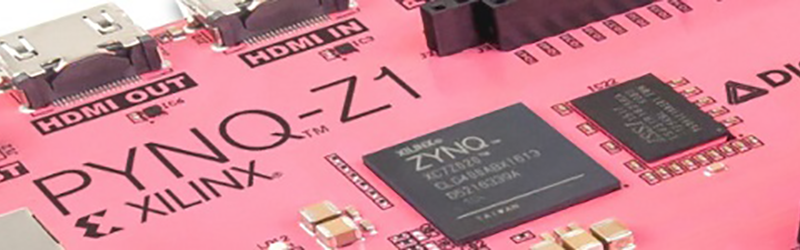
\includegraphics[width=8cm]{PIC/pynqcore}}
	\caption{PYNQ Z1 Core}
	\label{PYNQ Z1 Core}
	\end{figure}


\subsection{Power Jumper}

PYNQ Z1 hat 2 \textbf{''Modi''} Form der spannungsversorgung, dass die brauchte Spannung versorgt wird.

Diese spannungsversorgung kann durch die Änderung des Power Jumpers geschafft werden.


	\begin{enumerate} 
	\item \textbf{USB} über Anschluss J14 (PROG oder UART)
	\item  \textbf{REG} über Anschluss J18 (External Power)\\
	\end{enumerate}

	\textbf{Hinweis1 :} Die Ausgangsspannung \textbf{AC} muss zwischen 7VDC und 15VDC sein.
	
	\textbf{Hinweis2 :} Wenn die Eingangsspannungen \textbf{>15VDC} sein, wird das Board beschädigt.



	\begin{figure}[H]
	\centering
	\subfloat{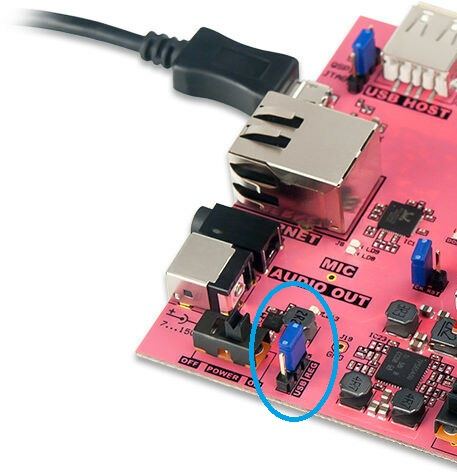
\includegraphics[width=5cm]{PIC/Jumper_Netzteil}}
	\caption{Power Jumper}
	\label{Power_Jumper}
	\end{figure}



\subsection{Programming Switching Jumper(Boot Jumper)}

Wird zum wählen des Bootmodus gesetzt. Das Board kann über SD-Karte, Quad SPI oder JTAG gebootet werden.

	\begin{figure}[H]
	\centering
	\subfloat{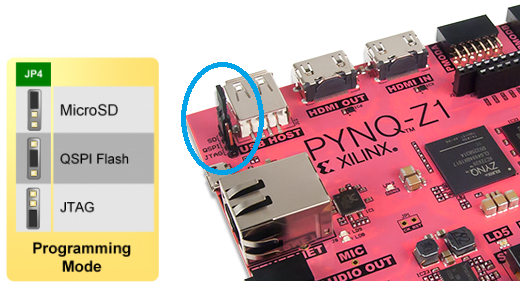
\includegraphics[width=5cm]{PIC/BootJumper}}
	\caption{BootJumper}
	\label{Boot_Jumperr}
	\end{figure}

Die drei Startmodi werden im folgenden Text beschrieben: 

	\begin{enumerate} 
	\item   \textit{microSD Boot Mode}
	
	Der PYNQ-Z1 unterstützt \textbf{Booting} von einer microSD-Karte, die in Anschluss \textbf{J9} eingesetzt ist.
	
	\item  \textit{Quad SPI Boot Mode}
	
	Der PYNQ-Z1 verfügt über einen integrierten 16-MB-Quad-SPI-Flash, von dem der Zynq booten kann.
	
	\item  \textit{JTAG Boot Mode}
	
	Wenn der Prozessor in den JTAG-Startmodus versetzt wird, wartet er, bis die Software mithilfe der Xilinx-Tools von einem Host-Computer geladen wird.\\
Nach dem Laden der Software kann die Software entweder mit der Ausführung beginnen oder mit dem Xilinx SDK zeilenweise durchlaufen werden.
	\end{enumerate}

\subsection{microSD Slot}

Der PYNQ-Z1 bietet einen microSD-Steckplatz\footnote{Slot} (J9) für \textit{''non-volatile''} externen Speicher sowie zum Booten des Zynq.
Der Steckplatz ist mit Bank 1/501 MIO [40-47] auch einschließlich Card Detect verbunden.

	\begin{figure}[H]
	\centering
	\subfloat{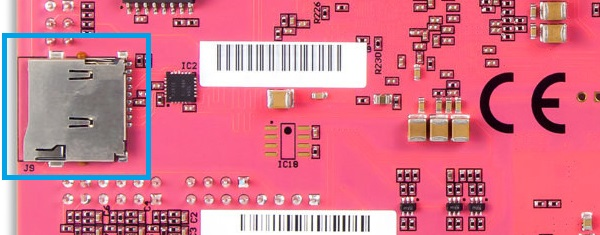
\includegraphics[width=7cm]{PIC/SDcard}}
	\caption{microSD Slot}
	\label{microSD_Slot}
	\end{figure}
	
	
\textbf{Hinweis:} Für das Betriebssystem wird mindestens eine\textbf{ Klasse-4 Karte} mit \textbf{8 GB Speicherplatz} empfohlen.

Informationen zum Einrichten und Verwendung der Speicherkarte finden Sie im Abschnitt Software und im Bereich \textbf{\nameref{Einrichtung_der_Speicherkarte}}.

\subsection{PMOD A/B}
\label{PMODE_PORTS}

Ein Pmod-Port ist eine offene 12-polige Schnittstelle, die von einer Reihe von Pmod-Peripheriegeräten unterstützt wird.\\

Typische Pmod-Peripheriegeräte sind:
	
	\begin{itemize}
		\item Sensoren (Spannung, Licht, Temperatur)
		\item Kommunikationsschnittstellen (Ethernet, seriell, WLAN, Bluetooth) 
		\item Eingangs- und Ausgangsschnittstellen (Tasten, Schalter, LEDs)
	\end{itemize}

		\begin{figure}[H]
			\centering
			\subfloat{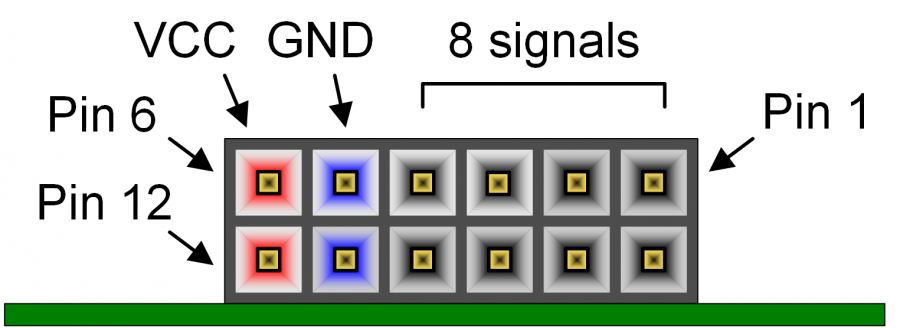
\includegraphics[width=7cm]{PIC/pynqPmod}}
			\qquad
			\subfloat{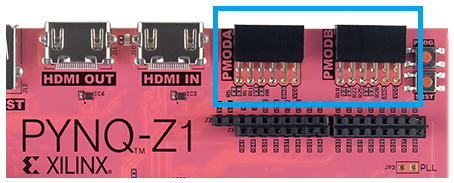
\includegraphics[width=7cm]{PIC/pmodport}}
			\caption{PYNQ PMODE Pins und PYNQ PMODE Ports }
			\label{fig:PYNQ_PMODE_PYNQ_PMODE_Ports}
		\end{figure}


	
High-Speed Pmod ports, Jeder 12 pins Pmod Port liefert zwei 3,3 VCC Signale (Pins 6 und 12), zwei Groundssignale (Pins 5 und 11) und 8 Logiksignale.

\textbf{Hinweis:} Da die Pins nicht gegen Kurzschluss oder Überspannung (>3.3V) geschützt sind, muss beim verdrahten
besonders aufgepasst werden.\\\\
Aufgrund der Verwendung dieser Komponente  im Projekt werden wirIn den folgenden Kapiteln und der \textbf{\nameref{Implementierung_des_Projeks}}-Abschnitt vollständig erklärt.


\subsection{Arduino / chipKIT Shield Header}
Der PYNQ-Z1 kann an Standard-Arduino und ChipKIT Shields angeschlossen werden, um die Funktionalität zu erweitern.
Der Shield Connector verfügt über 49 Pins, die für allgemeine digitale E / A mit dem Zynq PL verbunden sind.

	\begin{figure}[H]
	\centering
	\subfloat{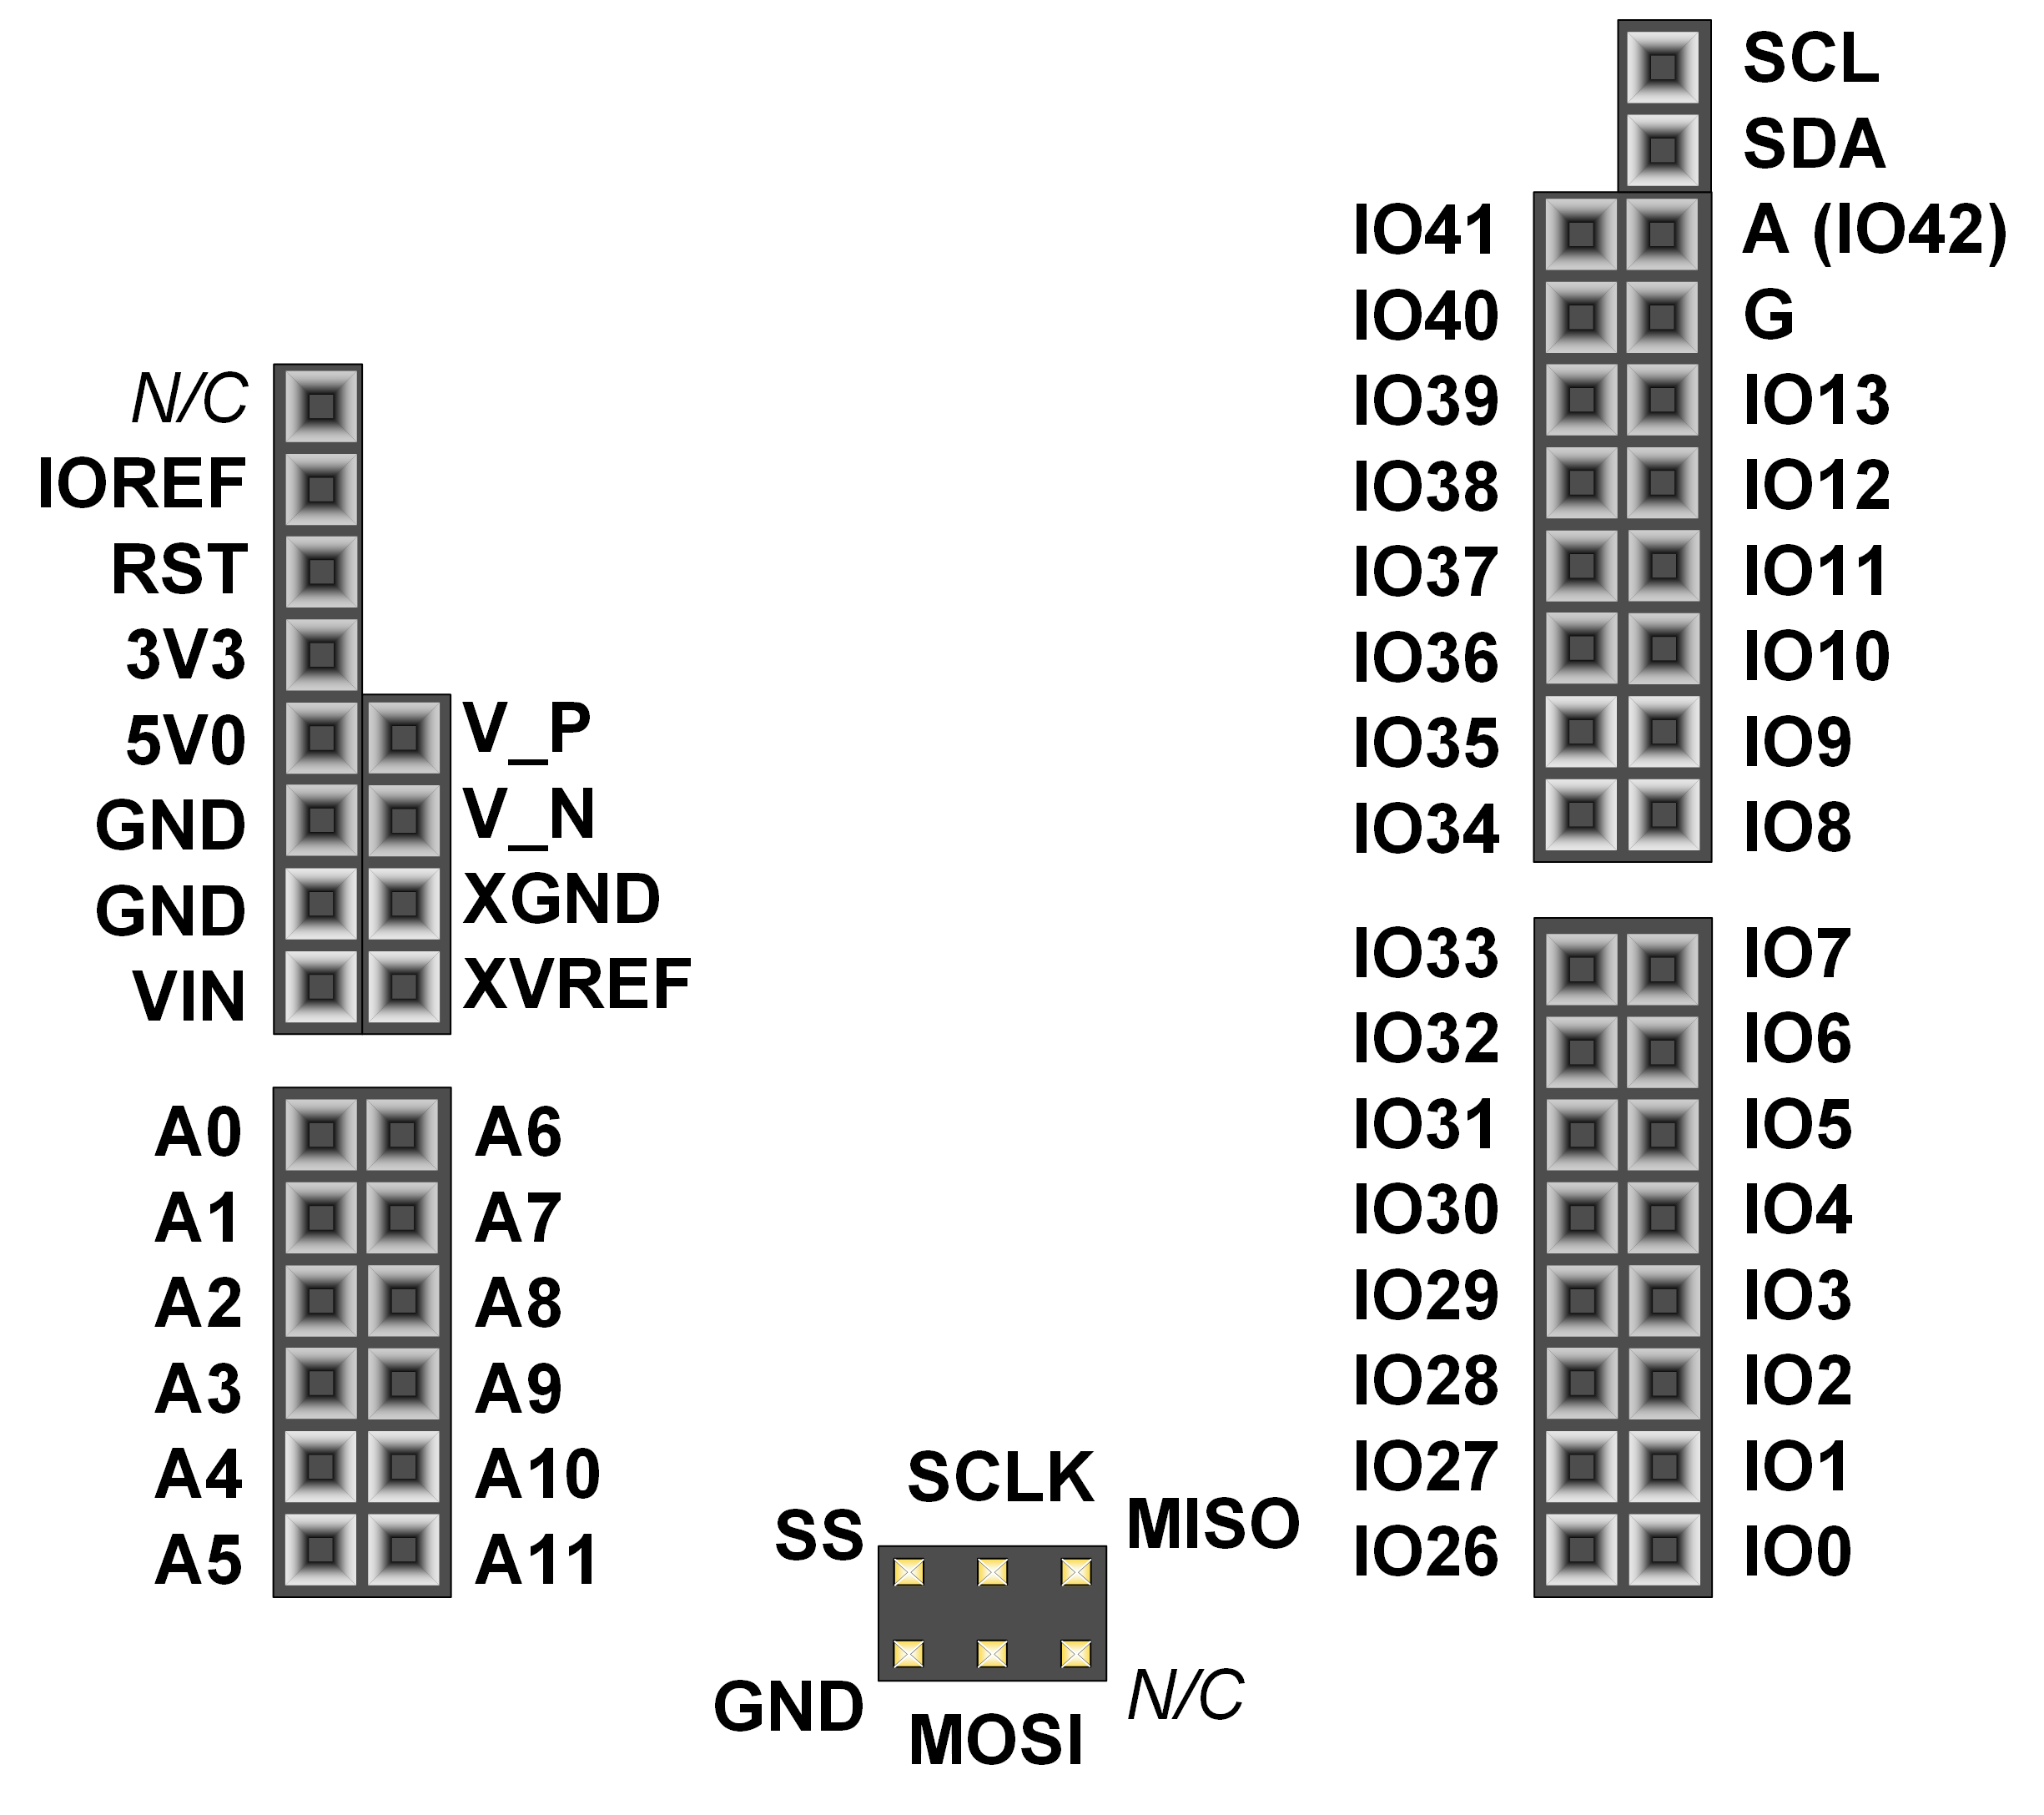
\includegraphics[width=7cm]{PIC/pynqz1shield}}
	\caption{Shield Pin Diagram}
	\label{fig:Shield_Pin_Diagram}
	\end{figure}

Aufgrund der Flexibilität von FPGAs können diese Pins für nahezu alles verwendet werden, einschließlich digitalem Lesen / Schreiben, SPI-Verbindungen, UART-Verbindungen, I2C\footnote{I-squared-C protocol}Verbindungen und PWM.

6 dieser Pins (mit AN0-AN5 bezeichnet) können auch als unsymmetrische Analogeingänge mit einem Eingangsbereich von 0 V bis 3,3 V verwendet werden, und weitere 6 (mit AN6-11 bezeichnet) können als differentielle Analogeingänge verwendet werden.\\

	\textbf{Hinweis1 :} Der PYNQ-Z1 ist \textbf{nicht} mit Shield kompatibel, die 5-V-Digital- oder Analogsignale ausgeben.
	
	\textbf{Hinweis2 :}  Mehr als \textbf{5 V} kann die Driving pins am PYNQ-Z1- Shield Connector beschädigen.



\subsection{Ethernet}
Der PYNQ-Z1 verwendet einen Realtek RTL8211E-VL PHY, um einen 10/100/1000 Ethernet-Port für die Netzwerkverbindung zu implementieren.

	\begin{figure}[H]
	\centering
	\subfloat{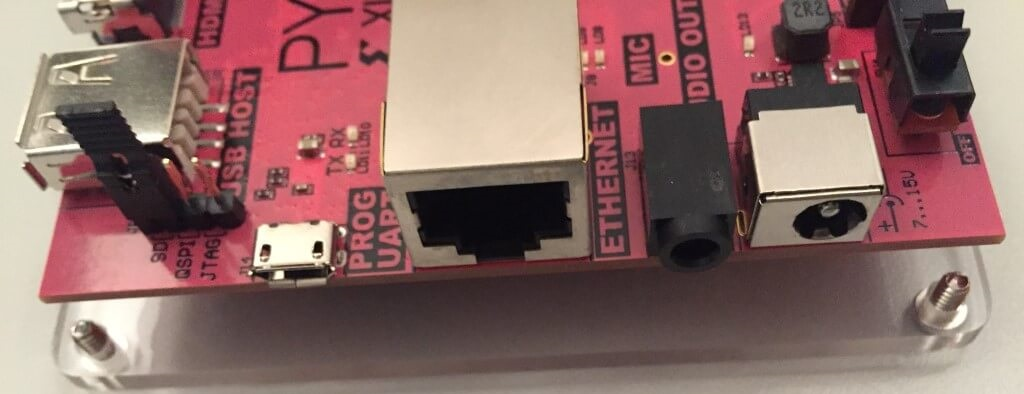
\includegraphics[width=7cm]{PIC/PYNQZ1Ethernet}}
	\caption{Ethernet}
	\label{fig:Ethernet}
	\end{figure}

Das Board versucht nach dem Anschalten über DHCP eine IP-Adresse zu erhalten und fällt auf 192.168.3.99/24 zurück, falls kein DHCP Server verfügbar ist.

\textbf{Hinweis:} IP-Adresse hängt von der Version des Image Files \textbf{pynq{\_}z1{\_}v2 .1 . img}, aber bei der Version 2.0 lautet 192.168.2.99 und es ist möglich, dass bei der Version 2.0 geändert werden kann.
	
Der PYNQ-Z1 enthält auch andere Komponenten wie MIC/AUDIO OUT, Schalter, Taster, RGB LEDs, u.s.w.\\\\

Weitere Informationen zu diesen Teilen finden Sie im PYNQ-Z1-Handbuch.




\section{Kamera - Ov7670}
Der OV7670 verwendet den RGB565-Modus mit 30 Bildern pro Sekunde und eine Erfassungsauflösung von 640 x 480, die im internen BRAM\footnote{BLOCK RAM} des 7Z020 des ZYNQ7-Chips gespeichert ist.
Der VGA-Controller liest die Daten auf der Leseseite und verwendet eine 12-Bit-Farbtiefe auf dem VGA-Schnittstellenbildschirm.\\
Die VGA-Auflösung beträgt ebenfalls 640x480. Die Kamera wird mit +3,3V versorgt.

		\begin{figure}[H]
			\centering
			\subfloat{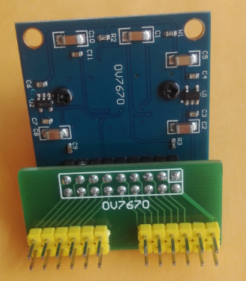
\includegraphics[width=4cm]{PIC/Ov7670camera_Back}}
			\qquad
			\subfloat{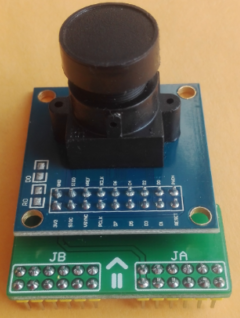
\includegraphics[width=3.45cm]{PIC/Ov7670camera_Front}}
			\caption{Kamera - Ov7670}
			\label{fig:Kamera - Ov7670}
		\end{figure}


\textbf{Hinweis: } 7Z020 verfügt über einen umfangreichen BLOCK RAM-Block, sodass Sie 640X480 = 307200 12-Bit-Nummern direkt speichern können, sodass kein externer Speicher für die Videopufferung verwendet wird.

Bemerkenswerte Eigenschaften dieser Kamera sind:
	\begin{itemize}
		\item Steuerung den SCB\footnote{Storz Communication Bus}-Busteil
		\item Broad stopband performance bis to 8 GHz
		\item Fast roll-off
		\item Connectorized package
	\end{itemize}







\section{VGA- D Adapter}
Es ist Kleine Platine mit 16 poligem Terminalblock ( Klemmleisten 3,81mm Raster) auf eine 3-reihige High Density Buchse für VGA\footnote{Video Graphics Array} Anwendungen.
VGA- D Adapter umfasst die Spezifikation einer analogen elektronischen Schnittstelle zur Übertragung von Bildern oder Videos zwischen unseren Board und Bildschirm sowie Spezifikationen für hierzu geeignete Stecker und Kabel.


		\begin{figure}[H]
			\centering
			\subfloat{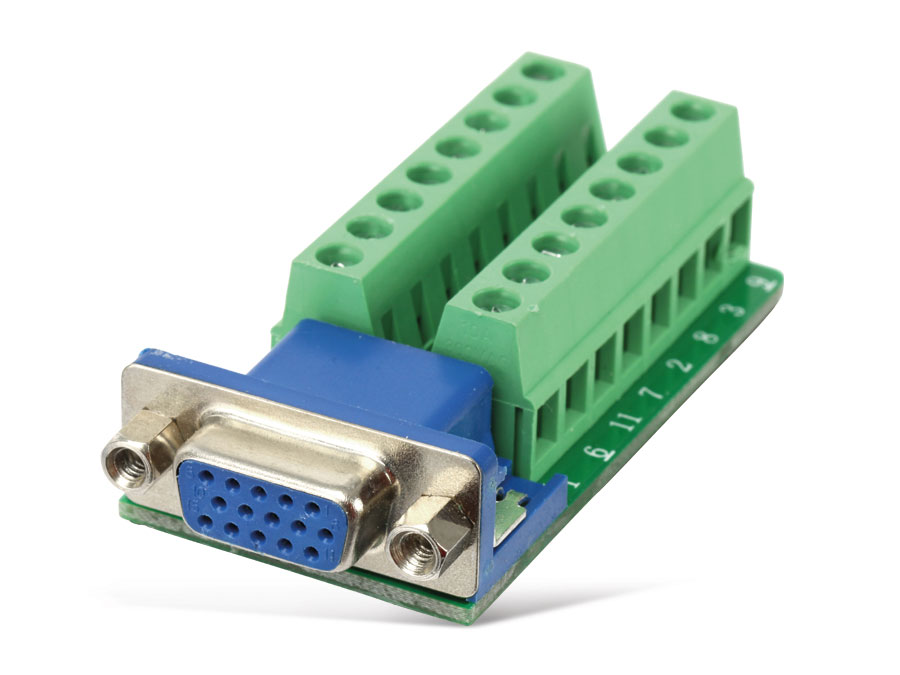
\includegraphics[width=5cm]{PIC/AdapterVGA2}}
			\qquad
			\subfloat{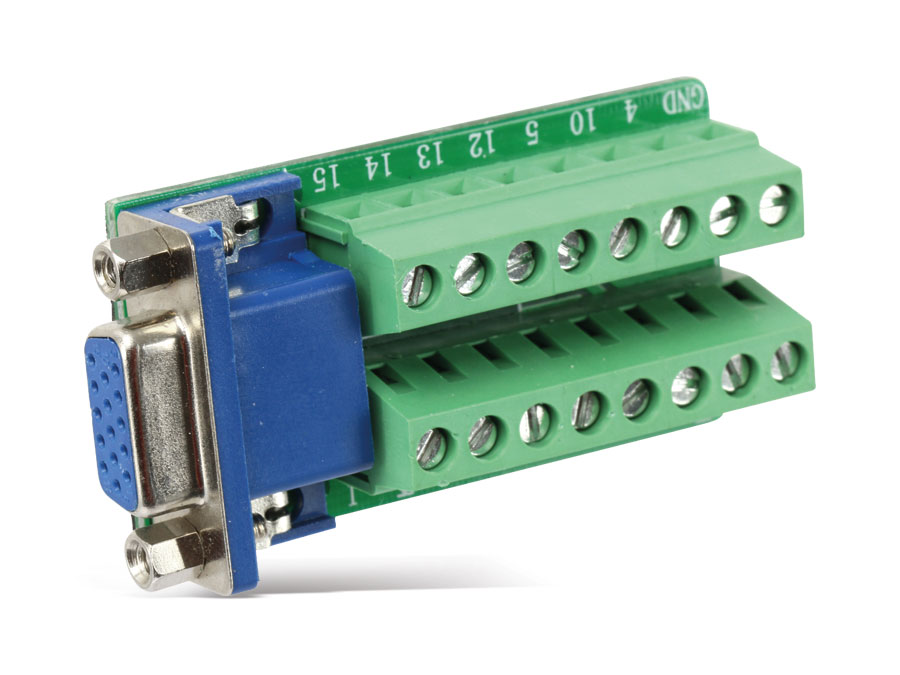
\includegraphics[width=5cm]{PIC/AdapterVGA1}}
			\caption{VGA D Adapter}
			\label{fig:VGA_Adapter}
		\end{figure}




	%------------------------------------------------
	%	3. Chapter
	%------------------------------------------------

\chapter{Softdware}

	
\section{Einrichtung der SDkarte}
\label{Einrichtung_der_SDkarte}


Mit dem folgenden Verfahren können Sie den Zynq von microSD mit einem Standard-\textbf{Zynq-Boot-Image} starten, das mit den Xilinx-Tools erstellt wurde:

	\begin{enumerate} 
	
		\item Formatieren Sie die microSD-Karte mit einem FAT32-Dateisystem.
		\item Kopieren Sie das mit Xilinx SDK erstellte \textbf{Zynq Boot Image} auf die microSD-Karte.
		\item Benennen Sie das Zynq-Boot-Image auf der microSD-Karte in\textbf{ BOOT.bin }um.
		\item Entnehmen Sie die microSD-Karte aus Ihrem Computer und stecken Sie sie in den Anschluss\textbf{ J9} des PYNQ-Z1.
		\item Schließen Sie eine\textbf{ Stromquelle} an den PYNQ-Z1 an und wählen Sie sie mit\textbf{ JP5 }aus.
		\item Stecken Sie einen einzelnen\textbf{ Jumper} auf \textbf{ JP4 } und schließen Sie die beiden oberen Stifte (mit der Bezeichnung „SD“) kurz.
		\item Schalten Sie die Karte ein. Das Board bootet nun das Image von der microSD-Karte.

	\end{enumerate}

	%------------------------------------------------
	%	4. Chapter
	%------------------------------------------------

\chapter{Implementierung des Projeks}
\label{Implementierung_des_Projeks}


\section{Hardwares Implementierung}

\subsection{Einstellung von Pmod port}
Wie im Abschnitt \textbf{\nameref{PMODE_PORTS}} schon erwähnt wurde, 


\section{HLS Software Implementierung}










	%------------------------------------------------
	%	Literaturverzeichnis
	%------------------------------------------------


\begin{thebibliography}{9}

\bibitem{PYNQ-Z1 Board} 
Xilinx PYNQ Z1 Board,
\\\texttt{https://blog.digilentinc.com/python-zynq-pynq-introducing-our-latest-collaborationl}

\bibitem{PYNQ-Z1} 
PYNQ Z1-Komponenten,
\\\texttt{https://buildmedia.readthedocs.org/media/pdf/pynq/v1.4/pynq.pdf}

\bibitem{PYNQ-Z1}
PYNQ Z1-Einrichtung,
\\\texttt{Pynq{\_}Labor{\_}Doku{\_}Jaschko{\_}Stolle.pdf}

\bibitem{Ov7670camera} 
Ov7670camera,
\\\texttt{http://www.alselectro.com/arduino-camera-ov7670.html}

\end{thebibliography}




\end{document}